% !TEX program = xelatex
\documentclass[UTF8,a4paper,zihao=-4,fontset=mac]{ctexart}
\usepackage[left=25mm,right=25mm,top=24mm,bottom=24mm,headheight=14pt]{geometry}
\usepackage{amsmath,amssymb,bm,booktabs,array,multirow,graphicx}
\usepackage{enumitem,float,caption,subcaption,fancyhdr,hyperref}
\usepackage[section]{placeins}
\usepackage{needspace}
\usepackage{tikz}
\usetikzlibrary{arrows.meta,positioning,calc,shapes.geometric}
\hypersetup{hidelinks,pdftitle={基于联合光线能量积分与分区优化的定日镜场设计},pdfauthor={}}
\captionsetup{font=small,labelfont=bf,labelsep=quad,skip=6pt}
\setlist{nosep,leftmargin=2em,topsep=3pt}
\ctexset{section={format=\large\bfseries,beforeskip=14pt,afterskip=8pt},
subsection={format=\normalsize\bfseries,beforeskip=10pt,afterskip=5pt},
subsubsection={format=\normalsize\bfseries,beforeskip=7pt,afterskip=3pt}}
\linespread{1.18}
\setlength{\parskip}{2pt}
\setlength{\emergencystretch}{2em}
\clubpenalty=10000
\widowpenalty=10000
\displaywidowpenalty=10000
\setlength{\textfloatsep}{12pt}
\setlength{\floatsep}{10pt}
\setlength{\intextsep}{10pt}
\makeatletter
\setlength{\@fptop}{0pt}
\setlength{\@fpsep}{12pt}
\setlength{\@fpbot}{0pt plus 1fil}
\makeatother
\renewcommand{\arraystretch}{1.2}
\pagestyle{fancy}
\fancyhf{}
\fancyfoot[C]{\small\thepage}
\renewcommand{\headrulewidth}{0pt}
\newcommand{\vect}[1]{\bm{#1}}
\newcommand{\dd}{\mathrm d}
\newcommand{\DNI}{\mathrm{DNI}}
\newcommand{\unitp}{\mathrm{kW}/\mathrm{m}^{2}}
\newcommand{\mean}[1]{\overline{#1}}
\newcommand{\QoneP}{35.2349}
\newcommand{\QoneJ}{0.56089}
\newcommand{\QoneOpt}{0.57632}
\newcommand{\QoneCos}{0.75647}
\newcommand{\QoneSB}{0.91669}
\newcommand{\QoneTrunc}{0.94831}
\newcommand{\QoneAt}{0.96516}
\newcommand{\QoneWidth}{6.0000}
\newcommand{\QoneHeight}{6.0000}
\newcommand{\QoneZ}{4.0000}
\newcommand{\QoneCount}{1745}
\newcommand{\QtwoP}{60.0582}
\newcommand{\QtwoJ}{0.49265}
\newcommand{\QtwoOpt}{0.50544}
\newcommand{\QtwoCos}{0.75470}
\newcommand{\QtwoSB}{0.84559}
\newcommand{\QtwoTrunc}{0.91323}
\newcommand{\QtwoAt}{0.96401}
\newcommand{\QtwoWidth}{7.0902}
\newcommand{\QtwoHeight}{7.0902}
\newcommand{\QtwoZ}{3.6451}
\newcommand{\QtwoCount}{2425}
\newcommand{\QthreeP}{60.0668}
\newcommand{\QthreeJ}{0.50212}
\newcommand{\QthreeOpt}{0.51517}
\newcommand{\QthreeCos}{0.75539}
\newcommand{\QthreeSB}{0.85986}
\newcommand{\QthreeTrunc}{0.91299}
\newcommand{\QthreeAt}{0.96411}
\newcommand{\QthreeWidth}{7.0902}
\newcommand{\QthreeHeight}{6.9402}
\newcommand{\QthreeZ}{3.6451}
\newcommand{\QthreeCount}{2404}
\newcommand{\QthreeTypes}{9}
\newcommand{\QthreeZTypes}{2}
\newcommand{\GainJ}{1.921}
\newcommand{\AreaSaving}{1.871}
\newcommand{\PairedDiff}{0.009466}
\newcommand{\PairedLow}{0.009444}
\newcommand{\LegacyP}{43.2059}
\newcommand{\ConvMax}{0.0109}


\begin{document}
\hypersetup{pageanchor=false}
\thispagestyle{empty}
\begin{center}
{\zihao{3}\bfseries 基于联合光线能量积分与分区优化的定日镜场设计}\par
\vspace{5mm}
{\large\bfseries 摘\quad 要}
\end{center}

定日镜场的单位面积产热能力同时受太阳位置、镜面姿态、镜间遮挡与集热器截断影响，扩大镜面或增加镜数并不一定带来同比例的热功率增长。针对圆形场地内的定日镜场设计，本文建立太阳圆盘与镜面面积上的联合光线能量积分模型，并在年平均输出热功率不低于 $60\,\mathrm{MW}$ 的约束下，分别求解统一镜型与异构镜型的参数化布局优化问题。

\textbf{针对问题一，}在东、北、天顶坐标系中直接计算太阳方向，以太阳中心方向与镜心指向集热器方向的角平分线确定镜面法向。对镜面面积和有限太阳圆盘联合进行扰乱 Sobol 采样，通过有限矩形求交识别阴影与反射遮挡，通过有限圆柱的首次相交识别有效接收光线。同一批光线同时计算余弦、遮挡和截断效率，避免重叠损失重复扣除。对附件 $1745$ 面镜及规定的 $60$ 个时刻复算，年平均光学效率为 \QoneOpt，年平均输出热功率为 \QoneP\,$\mathrm{MW}$，单位镜面面积年平均输出为 \QoneJ\,$\unitp$。

\textbf{针对问题二，}将塔址、统一镜面尺寸、安装高度以及交错布局参数作为设计变量，采用容量筛选、完整光线追踪和收益排序删镜相结合的求解方法，在已有坐标改进方案上补充塔址与环带相位的多起点搜索。得到 \QtwoCount\ 面统一定日镜，尺寸为 $\QtwoWidth\,\mathrm m\times\QtwoHeight\,\mathrm m$，安装高度为 $\QtwoZ\,\mathrm m$；年均输出为 \QtwoP\,$\mathrm{MW}$，单位面积年均输出为 \QtwoJ\,$\unitp$，全部几何约束通过检查。

\textbf{针对问题三，}按径向距离和方位将镜场划分为六组，加入安装高度剖面比较与完整双向坐标搜索，并比较区域统一镜型以减少零散规格。最终设计包含 \QthreeCount\ 面镜，年均输出为 \QthreeP\,$\mathrm{MW}$，单位面积年均输出为 \QthreeJ\,$\unitp$，较统一镜型提高 \GainJ\%。两类设计分别经每镜每时刻 $4096$ 条光线、$4$ 组独立随机化复核，年均功率的单侧 $95\%$ 数值下界均超过额定值。

进一步通过光线数收敛、独立实现对照及太阳视半径、塔身半径、镜面斜率误差的敏感性实验检验模型。结果表明，联合能量积分能够保持光学损失与输出功率之间的一致性，分区异构设计能够改善镜面面积的利用。所给方案为明确物理假设和搜索范围内的可行改进解。

\vspace{3mm}
\noindent\textbf{关键词：}定日镜场；几何光学；扰乱 Sobol 积分；约束优化；异构镜面

\clearpage
\setcounter{page}{1}
\hypersetup{pageanchor=true}
\section{问题重述}
\subsection{背景与已知条件}
塔式太阳能光热电站利用定日镜将太阳辐射反射至吸收塔顶部的集热器，获得用于储热和发电的热能。镜场面积、镜面尺寸及镜间距离共同限制可安装的镜数，而太阳位置随日期与时刻变化，使每面镜的有效产热能力具有显著的时空差异。因此，镜场设计需要同时协调容量、光学效率与用地条件。

题目给定场址为东经 $98.5^\circ$、北纬 $39.4^\circ$、海拔 $3000\,\mathrm m$，可建设区域是半径 $350\,\mathrm m$ 的圆盘。坐标原点位于场地中心，$x$ 轴向东、$y$ 轴向北、$z$ 轴向上。集热器为高 $8\,\mathrm m$、直径 $7\,\mathrm m$ 的圆柱形外表受光式结构，其中心离地 $80\,\mathrm m$；塔周 $100\,\mathrm m$ 内不安装定日镜。

定日镜为上下边保持水平的平面矩形，宽、高均在 $2$ 至 $8\,\mathrm m$ 之间，宽度不小于高度，安装高度在 $2$ 至 $6\,\mathrm m$ 之间，且旋转中不得触地。相邻底座须留出镜面宽度之外至少 $5\,\mathrm m$ 的间距。本文严格按每月 $21$ 日的 $9{:}00$、$10{:}30$、$12{:}00$、$13{:}30$、$15{:}00$ 共 $60$ 个时刻等权计算年均指标\cite{problem}。

\subsection{需要解决的问题}
\begin{enumerate}[label=（\arabic*）]
\item 给定塔址为圆心、镜面尺寸为 $6\,\mathrm m\times6\,\mathrm m$、安装高度为 $4\,\mathrm m$ 以及附件镜心坐标，计算逐月与年平均光学效率、输出热功率和单位镜面面积输出热功率。
\item 所有镜面尺寸和安装高度相同，联合设计塔址、镜型、镜数及位置，在年均热功率达到 $60\,\mathrm{MW}$ 时，使单位镜面面积年均热功率尽量大。
\item 放开镜面尺寸及安装高度的统一限制，在相同额定功率要求下，利用异构镜面进一步提高单位面积年均热功率。
\end{enumerate}

\section{问题分析与总体思路}
\subsection{从单镜效率到全场能量}
问题一是定场计算，需要在真实几何下同时处理余弦、大气衰减、阴影、遮挡和截断等主要光学损失\cite{zhang,farges}。阴影发生在太阳至镜面的入射光路上，遮挡发生在镜面至集热器的反射光路上，截断则发生于反射光束与有限集热器不能完全重合时。三类几何损失作用在同一束光线上，彼此具有相关性。若分别估计损失率后独立相乘，重叠区域可能被重复扣除，且无法正确计算条件截断效率。

为此，本文从镜面采样点出发，先判断朝向太阳的可见性，再判断反射光线的可见性，最后判断首次命中的接收表面，建立统一的能量统计过程。该模型也作为问题二、三的共同评价器，保证设计比较使用相同物理标准。

\subsection{从容量满足到面积利用}
问题二是镜数可变的混合约束优化。大镜面能提高几何采光面积，却也扩大维护间距、反射光斑和遮挡范围；塔址向南平移有利于增加北侧高余弦效率区域，但也会改变可用区域形状和远距离反射损失。因而不能仅凭“镜面越大越好”或“塔越靠南越好”确定方案。

问题三进一步引入数千个镜面的尺寸和高度自由度。直接逐镜全维搜索会产生大量不可行试探。本文先按距离和方位构造六个区域，寻找不同区域的面积调整方向，再进行局部细化。对于容量不足的高效率试探，补充合适镜面恢复容量；对于容量富余的试探，删去低收益镜面以压缩面积。

\begin{figure}[htbp]
\centering
\begin{tikzpicture}[node distance=7mm and 8mm,>=Latex,
box/.style={draw,rounded corners=1pt,align=center,text width=42mm,minimum height=12mm,font=\small}]
\node[box] (input) {题目参数与附件坐标\\60 个规定时刻};
\node[box,right=of input] (geom) {太阳方向与镜面姿态\\有限太阳圆盘采样};
\node[box,right=of geom] (trace) {阴影、遮挡、首次命中\\联合能量积分};
\node[box,below=of input] (qone) {问题一：定场计算\\月均与年均指标};
\node[box,below=of geom] (qtwo) {问题二：统一镜型\\容量恢复与面积压缩};
\node[box,below=of trace] (qthree) {问题三：分区异构\\补镜、交换与微调};
\node[box,below=of qtwo,text width=70mm] (check) {独立随机化复核、约束检查\\收敛与物理假设敏感性};
\draw[->] (input)--(geom);\draw[->] (geom)--(trace);
\coordinate (branch) at ($(trace.south)+(0,-3.5mm)$);
\draw (trace.south)--(branch);
\draw[->] (branch)-|(qone.north);
\draw[->] (branch)-|(qtwo.north);
\draw[->] (branch)--(qthree.north);
\draw[->] (qone.south)|-(check.west);
\draw[->] (qtwo)--(check);\draw[->] (qthree.south)|-(check.east);
\end{tikzpicture}
\caption{三问共享光学评价器的求解流程}
\end{figure}

\section{模型假设与符号说明}
\subsection{模型假设}
\begin{enumerate}[label=假设\arabic*：,leftmargin=4em]
\item 场地为水平面，空气与镜面反射性质在规定时刻内稳定；不引入云量、积灰、风载、热损和热电转换效率，所计算功率为题目定义的集热器接收热功率。
\item 直接采用附录中的当地时间计算太阳时角，以 $2023$ 年 $3$ 月 $21$ 日为春分零日，不另做北京时间换算；所有 $60$ 个时刻等权，不按日长或月份天数重新加权。
\item 基准太阳为均匀辐亮度圆盘，视半径取 $4.65\,\mathrm{mrad}$；镜面为理想平面镜，控制系统使太阳中心光线经镜心反射后指向集热器中心，基准不加入斜率或跟踪误差。
\item 将外表受光式圆柱的侧面视为有效受光面，上下端面只作为几何遮挡边界。集热器范围为 $z\in[76,84]\,\mathrm m$，吸收塔高度 $80\,\mathrm m$ 指集热器中心高度。
\item 题目未给塔身半径，基准取半径 $2\,\mathrm m$、高度 $76\,\mathrm m$ 的竖直圆柱；它与集热器本体均参与阴影判断。太阳视半径和塔身尺寸的影响另作敏感性分析。
\item 对新设计采用保守边界：镜面外接圆完全位于场地内，并完全避开塔周禁区；异构镜对的最小底座间距按两者较大宽度加 $5\,\mathrm m$ 判定。问题一原样使用附件坐标。
\end{enumerate}

这些假设区分了题目给定常数和为闭合模型补充的物理量。特别地，太阳锥角不以随机制造误差代替，平面镜也不改为理想聚焦曲面，从而保留了有限光束的截断效应。

\Needspace{17\baselineskip}
\subsection{主要符号}
\begin{table}[H]
\centering\small
\caption{主要符号与单位}
\begin{tabular}{p{27mm}p{98mm}l}
\toprule
符号 & 含义 & 单位\\\midrule
$\mathcal T$，$N$ & 规定计算时刻集合、定日镜数目 & ---\\
$\vect c_i=(x_i,y_i,z_i)$ & 第 $i$ 面镜的中心位置，$z_i$ 为安装高度 & m\\
$w_i,h_i,A_i$ & 镜面宽度、高度与面积，$A_i=w_ih_i$ & m，m$^2$\\
$\vect T=(x_T,y_T,80)$ & 集热器中心，$(x_T,y_T)$ 为塔址 & m\\
$\vect s,\vect s'$ & 太阳中心方向、太阳圆盘采样方向单位向量 & ---\\
$\vect t_i,\vect n_i$ & 镜心指向接收中心的单位向量、镜面单位法向 & ---\\
$\vect u_i,\vect v_i$ & 镜面水平宽度方向、高度方向单位向量 & ---\\
$\DNI_t$ & 第 $t$ 个时刻的法向直接辐照度 & kW/m$^2$\\
$\eta_{\rm cos},\eta_{\rm sb}$ & 余弦效率、阴影遮挡效率 & ---\\
$\eta_{\rm at},\eta_{\rm trunc},\eta_{\rm ref}$ & 大气透射率、截断效率、反射率 & ---\\
$P_t,\mean P,J$ & 瞬时全场热功率、年均热功率、单位面积年均功率 & kW，kW/m$^2$\\
$K,M$ & 每镜每时刻采样数、独立随机化组数 & ---\\\bottomrule
\end{tabular}
\end{table}

\section{联合光线能量积分模型}
\subsection{太阳方向与辐照度}
设纬度为 $\varphi=39.4^\circ$，$D$ 为相对春分的日数，太阳赤纬和时角满足
\begin{equation}
\sin\delta=\sin\!\left(\frac{2\pi D}{365}\right)\sin23.45^\circ,
\qquad \omega=\frac{\pi}{12}(ST-12).
\end{equation}
在东、北、天顶坐标系中，太阳中心方向直接写为
\begin{equation}
\vect s=\begin{bmatrix}
-\cos\delta\sin\omega\\
\sin\delta\cos\varphi-\cos\delta\sin\varphi\cos\omega\\
\sin\delta\sin\varphi+\cos\delta\cos\varphi\cos\omega
\end{bmatrix}.
\label{eq:sun}
\end{equation}
其中 $s_z=\sin\alpha_s$。上午 $\omega<0$ 时 $s_x>0$，下午则 $s_x<0$，可直接满足太阳位于东、西两侧的方向关系；无需从反余弦函数恢复方位角象限。

法向直接辐照度采用题目附录公式：
\begin{align}
\DNI_t&=1.366\left[a+b\exp\left(-\frac{c}{s_z}\right)\right],\\
a&=0.4237-0.00821(6-H)^2,\nonumber\\
b&=0.5055+0.00595(6.5-H)^2,\nonumber\\
c&=0.2711+0.01858(2.5-H)^2.\nonumber
\end{align}
式中 $H=3\,\mathrm{km}$，故 $a=0.34981$、$b=0.5783875$、$c=0.275745$。所有规定时刻太阳均高于地平线。镜心至集热器中心距离为 $d_i=\|\vect T-\vect c_i\|$，大气透射率为
\begin{equation}
\eta_{{\rm at},i}=0.99321-1.176\times10^{-4}d_i+1.97\times10^{-8}d_i^2,
\qquad d_i\le1000\,\mathrm m.
\label{eq:at}
\end{equation}
反射率取题目给出的 $\eta_{\rm ref}=0.92$。同一布局的 $d_i$ 不随时刻改变，可在时间循环外预计算。

\subsection{满足镜边水平约束的反射几何}
令镜心指向集热器中心的单位向量为
\begin{equation}
\vect t_i=\frac{\vect T-\vect c_i}{d_i},\qquad
\vect n_i=\frac{\vect s+\vect t_i}{\|\vect s+\vect t_i\|}.
\label{eq:normal}
\end{equation}
则太阳中心光线的反射方向满足
\begin{equation}
2(\vect n_i\cdot\vect s)\vect n_i-\vect s=\vect t_i,
\end{equation}
从而严格符合题目中的镜心瞄准要求。在 $n_{ix}^2+n_{iy}^2>0$ 时，取
\begin{equation}
\vect u_i=\frac{(-n_{iy},n_{ix},0)}{\sqrt{n_{ix}^2+n_{iy}^2}},
\qquad \vect v_i=\vect n_i\times\vect u_i.
\end{equation}
若法向竖直，可取 $\vect u_i=(1,0,0)$。由于 $u_{iz}=0$，宽度方向始终水平，满足上下两条镜边平行地面的限制。镜面任意点表示为
\begin{equation}
\vect p_i(\xi,\zeta)=\vect c_i+\xi w_i\vect u_i+\zeta h_i\vect v_i,
\qquad -\tfrac12\le\xi,\zeta\le\tfrac12.
\end{equation}
一面镜在同一时刻只有一个宏观法向 $\vect n_i$，不对不同采样点分别重新瞄准。否则会把平面镜错误地处理成具有理想聚焦能力的曲面镜。

\subsection{有限太阳圆盘与能量权重}
设太阳视半径为 $\alpha_\odot$，在垂直于 $\vect s$ 的平面内取正交单位基 $\vect a,\vect b$。令 $U,V\in[0,1]$，采用均匀投影立体角采样：
\begin{equation}
\sin\theta=\sin\alpha_\odot\sqrt U,\quad \psi=2\pi V,
\quad \vect s'=\cos\theta\vect s+\sin\theta(\cos\psi\vect a+\sin\psi\vect b).
\end{equation}
均匀辐亮度太阳盘向中心法向平面贡献的能量与 $\cos\theta\,\dd\Omega$ 成正比，因而上述采样与 $\DNI$ 的定义相匹配。镜面上的相对能量权重为
\begin{equation}
q=\frac{\max(0,\vect n_i\cdot\vect s')}{\vect s\cdot\vect s'}.
\label{eq:weight}
\end{equation}
分母是太阳中心法向投影修正项。当太阳盘收缩为一点时，式\eqref{eq:weight}退化为通常的余弦效率 $\vect n_i\cdot\vect s$。

太阳光的入射传播方向为 $-\vect s'$，从镜面点出发的反射方向为
\begin{equation}
\vect r=2(\vect n_i\cdot\vect s')\vect n_i-\vect s'.
\label{eq:reflection}
\end{equation}
将 $(\xi,\zeta,U,V)$ 作为联合积分变量，使用扰乱 Sobol 点覆盖镜面面积与太阳圆盘。基准光学积分本质上为四维；实现同时预留两维正态变量，用于斜率误差敏感性情景。Sobol 低差异点用于提高空间覆盖均匀性，独立扰乱则用于估计数值积分的不确定性\cite{sobol,owen}。

\subsection{阴影、遮挡与有限物体求交}
\subsubsection{矩形镜面求交}
从点 $\vect p$ 沿单位方向 $\vect d$ 发出射线，与第 $j$ 面镜所在平面相交的参数为
\begin{equation}
\lambda_j=\frac{(\vect c_j-\vect p)\cdot\vect n_j}{\vect d\cdot\vect n_j}.
\end{equation}
当分母非零、$\lambda_j>0$，且交点相对镜心的向量 $\vect a_j=\vect p+\lambda_j\vect d-\vect c_j$ 满足
\begin{equation}
|\vect a_j\cdot\vect u_j|\le\frac{w_j}{2},\qquad
|\vect a_j\cdot\vect v_j|\le\frac{h_j}{2},
\label{eq:rect}
\end{equation}
则射线与有限矩形相交。平行或仅在射线反向相交的情况均排除。

判断入射阴影时，从镜面点沿 $+\vect s'$ \textbf{朝向太阳}追踪；若遇到其他镜面、塔身或集热器本体，则该点不能接收此方向的太阳光。这里查询方向与光子传播方向相反。反射遮挡则沿 $\vect r$ 追踪，检查其他镜面和位于集热器之前的塔身。对于有效受光射线，集热器位于 $z\ge76\,\mathrm m$，镜面远低于这一高度，因此向上反射射线遇到的其他镜面必在接收器之前。

\subsubsection{圆柱首次相交与截断}
取圆柱轴线为 $(x_T,y_T)$，半径 $R=3.5\,\mathrm m$。对于射线 $\vect p+\lambda\vect r$，令 $X=p_x-x_T$、$Y=p_y-y_T$，侧面求交满足
\begin{equation}
(r_x^2+r_y^2)\lambda^2+2(Xr_x+Yr_y)\lambda+X^2+Y^2-R^2=0.
\end{equation}
只保留正根且交点高度在 $[76,84]\,\mathrm m$ 内的解；同时计算与 $z=76$ 和 $z=84$ 两端面圆盘的正向交点。在所有候选中取最小的正 $\lambda$，仅首次命中侧面时记为有效接收。

该判定尤其影响远处平面镜的上下边缘光线。若光线先进入底面再穿出侧面，实际首次接触的是非受光端面，不能因为后续存在侧面交点而计入接收。塔身采用相同圆柱求交方法，其半径和上下界分别为 $2\,\mathrm m$ 与 $[0,76]\,\mathrm m$。

\subsection{相关损失下的效率与功率}
对第 $i$ 面镜、第 $t$ 个时刻，记第 $k$ 条光线的权重为 $q_k$。令 $I_k^{\rm in}$、$I_k^{\rm out}$ 分别表示入射与反射光路畅通，$I_k^{\rm rec}$ 表示首次命中集热器侧面。定义三个能量和：
\begin{align}
C_{it}&=\sum_{k=1}^{K}q_k,\\
S_{it}&=\sum_{k=1}^{K}q_kI_k^{\rm in}I_k^{\rm out},\\
H_{it}&=\sum_{k=1}^{K}q_kI_k^{\rm in}I_k^{\rm out}I_k^{\rm rec}.
\end{align}
同一条光线只需记录“是否被遮挡”，多个遮挡物的覆盖区域按布尔并集处理，不累加重复损失面积。于是
\begin{equation}
\eta_{{\rm cos},it}=\frac{C_{it}}{K},\quad
\eta_{{\rm sb},it}=\frac{S_{it}}{C_{it}},\quad
\eta_{{\rm trunc},it}=\frac{H_{it}}{S_{it}},
\label{eq:eta}
\end{equation}
零分母时相应效率按零处理。特别地，截断效率以\textbf{通过阴影和遮挡后的能量}为分母，与题目定义一致。三者乘积满足能量恒等式
\begin{equation}
\eta_{{\rm cos},it}\eta_{{\rm sb},it}\eta_{{\rm trunc},it}=\frac{H_{it}}{K}.
\end{equation}
因此，单镜与全场瞬时热功率分别为
\begin{equation}
P_{it}=\DNI_t A_i\eta_{{\rm at},i}\eta_{\rm ref}\frac{H_{it}}{K},
\qquad P_t=\sum_{i=1}^{N}P_{it}.
\label{eq:power}
\end{equation}
这一表达式把余弦、阴影、遮挡和截断的相关性保留到最终能量计算中。

\subsection{统计口径与空间加速}
设总镜面面积 $A=\sum_i A_i$，则月均热功率、年均热功率与优化目标为
\begin{equation}
\mean P_m=\frac15\sum_{t\in\mathcal T_m}P_t,\qquad
\mean P=\frac1{60}\sum_{t\in\mathcal T}P_t,\qquad J=\frac{\mean P}{A}.
\label{eq:average}
\end{equation}
场均效率采用面积加权。例如
\begin{equation}
\eta_{{\rm field},t}=\frac1A\sum_i A_i\eta_{it},\qquad
\mean\eta_{{\rm field},m}=\frac15\sum_{t\in\mathcal T_m}\eta_{{\rm field},t}.
\end{equation}
同尺寸镜场中面积加权等于算术平均，异构镜场则必须保留面积权重。本文各表的平均效率分别平均；不能将这些平均效率再次相乘作为年均光学效率，也不能把年均 $\DNI$ 与年均光学效率相乘代替式\eqref{eq:average}。

逐镜枚举全部遮挡物的代价约为 $O(60KN^2)$。由于基准入射逆向射线和反射射线均向上，射线高于场内最高镜面边缘后不可能再次遇镜。设出发镜最低高度为 $z_i^{-}$，最高镜面边缘为 $z_{\max}^{+}$，有效向上角下界为 $\beta_i>0$，可用
\begin{equation}
L_i=\frac{z_{\max}^{+}-z_i^{-}}{\tan\beta_i}+\rho_i+\max_j\rho_j,
\qquad \rho_i=\tfrac12\sqrt{w_i^2+h_i^2}
\end{equation}
构造保守的二维搜索半径。再用镜面包围球和光锥包络筛除不可能命中的镜对，最后执行精确求交。$\beta_i$ 同时考虑太阳角、目标仰角和太阳锥角；斜率误差扩大光锥包络，若向上角下界失效，则回退到全镜对计算。该方法不依赖固定最近镜数或任意邻域半径。

\section{问题一：给定镜场的热功率计算}
\subsection{数据处理与求解设置}
读取附件可得 $N=1745$，坐标不存在缺失值，全部镜面采用 $6\,\mathrm m\times6\,\mathrm m$、安装高度 $4\,\mathrm m$、塔址 $(0,0)$，总面积为 $62820\,\mathrm{m}^2$。不移动、剔除或补充附件镜面，以保证问题一回答的是给定镜场本身。

对全部 $60$ 个时刻独立构造镜面姿态。最终每镜每时刻使用 $K=4096$ 个采样点，并以四个不同随机种子独立扰乱。先合并各组接收能量与可见能量，再计算条件效率，避免直接平均条件比值带来的偏差。月均结果见表\ref{tab:q1month}。

\begin{table}[H]
\centering\small
\caption{问题一每月 21 日平均光学效率及输出热功率}\label{tab:q1month}
\begin{tabular}{lrrrrrr}
\toprule
日期 & $\mean\eta$ & $\mean\eta_{\rm cos}$ & $\mean\eta_{\rm sb}$ & $\mean\eta_{\rm trunc}$ & $\mean P$/MW & $J$/($\unitp$)\\\midrule
1 月 21 日 & 0.53709 & 0.71994 & 0.90008 & 0.95556 & 29.4124 & 0.46820\\
2 月 21 日 & 0.56381 & 0.74044 & 0.91802 & 0.94940 & 33.3981 & 0.53165\\
3 月 21 日 & 0.58299 & 0.76114 & 0.92303 & 0.94565 & 36.4324 & 0.57995\\
4 月 21 日 & 0.60008 & 0.77934 & 0.92596 & 0.94389 & 38.7978 & 0.61760\\
5 月 21 日 & 0.61034 & 0.78932 & 0.92777 & 0.94387 & 40.0641 & 0.63776\\
6 月 21 日 & 0.61367 & 0.79236 & 0.92841 & 0.94404 & 40.4537 & 0.64396\\
7 月 21 日 & 0.61022 & 0.78921 & 0.92775 & 0.94386 & 40.0506 & 0.63755\\
8 月 21 日 & 0.59938 & 0.77864 & 0.92584 & 0.94392 & 38.7085 & 0.61618\\
9 月 21 日 & 0.58207 & 0.76009 & 0.92289 & 0.94580 & 36.2922 & 0.57772\\
10 月 21 日 & 0.56118 & 0.73784 & 0.91684 & 0.95012 & 32.9676 & 0.52480\\
11 月 21 日 & 0.53428 & 0.71820 & 0.89786 & 0.95595 & 29.0136 & 0.46185\\
12 月 21 日 & 0.52079 & 0.71108 & 0.88584 & 0.95766 & 27.2279 & 0.43343\\
\bottomrule
\end{tabular}
\par\vspace{3pt}\begin{minipage}{.95\linewidth}\footnotesize 各项效率为五个规定时刻的面积加权均值，效率无量纲；功率先逐镜求和再对时刻平均。\end{minipage}
\end{table}


\subsection{年平均结果与季节性解释}
问题一的年平均光学效率为 \QoneOpt，余弦效率为 \QoneCos，阴影遮挡效率为 \QoneSB，截断效率为 \QoneTrunc；年平均输出热功率为 \QoneP\,$\mathrm{MW}$，单位面积年均输出为 \QoneJ\,$\unitp$。大气透射率的场均值为 \QoneAt，由于镜心与塔址固定，该指标不随月份变化。

\begin{figure}[htbp]
\centering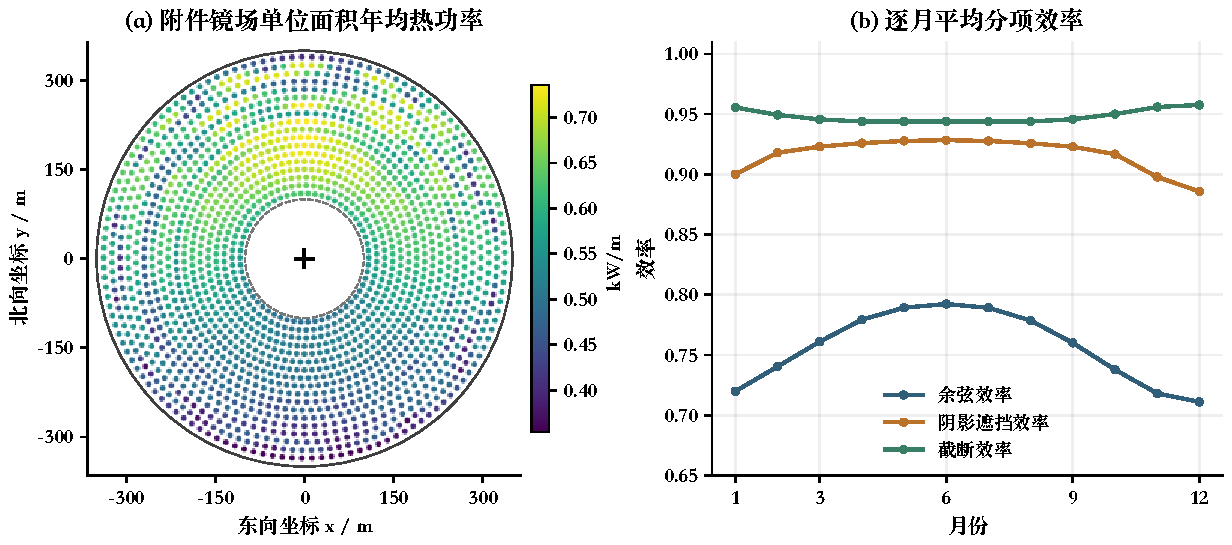
\includegraphics[width=.96\linewidth]{figures/q1_analysis.pdf}
\caption{给定镜场的空间产热差异及逐月光学效率}
\label{fig:q1}
\end{figure}

从图\ref{fig:q1}可见，镜场的单位面积年均产热具有明显方位差异。这是因为太阳主要位于南侧天空，北侧镜面指向集热器的方向通常与太阳方向更接近，从而获得较高余弦效率；同时，远距离镜面还受大气衰减和光斑扩展影响，不能只按“越北越优”排列。

夏季太阳高度较高，$\DNI$ 与余弦效率整体提高，镜面和塔身投影阴影较短；冬季相反，早晚时刻的低太阳高度使阴影损失更明显。截断效率为条件效率，它还取决于遮挡后留下的光线分布，因此其月度变化不必与余弦效率同向。这也说明用全年固定的阴影遮挡效率和截断效率会掩盖真实季节性。

本镜场年均功率距离额定 $60\,\mathrm{MW}$ 尚有较大差距。问题一较高的单位面积产热并不代表其可作为问题二的可行设计，后续优化必须在额定容量约束下重新权衡密度与光学损失。

\section{问题二：统一镜型的约束优化}
\subsection{优化模型与几何约束}
令设计变量为 $\mathcal F=\{(x_T,y_T),N,(x_i,y_i)_{i=1}^N,w,h,z\}$，统一镜型优化写为
\begin{equation}
\max_{\mathcal F} J(\mathcal F)=\frac{\mean P(\mathcal F)}{Nwh},
\qquad \mean P(\mathcal F)\ge60000\,\mathrm{kW}.
\label{eq:opt}
\end{equation}
其中功率由式\eqref{eq:power}逐镜逐时刻计算。保守几何约束为
\begin{equation}
\left\{\begin{aligned}
&2\le h\le w\le8,\quad 2\le z\le6,\quad z-h/2>0,\\
&\sqrt{x_i^2+y_i^2}+\rho\le350,\\
&\sqrt{(x_i-x_T)^2+(y_i-y_T)^2}-\rho\ge100,\\
&\sqrt{(x_i-x_j)^2+(y_i-y_j)^2}\ge w+5,\quad i\ne j,\\
&x_T^2+y_T^2\le350^2,\qquad N\in\mathbb N^+,
\end{aligned}\right.
\label{eq:constraints}
\end{equation}
其中 $\rho=\sqrt{w^2+h^2}/2$。镜面最低离地高度使用 $z-h/2$，这是对所有俯仰角均不触地的充分条件。镜间距使用平面底座距离，不将安装高度差错误地计入车辆通行间距。

目标函数含有镜数变化和光线遮挡边界，通常不光滑且非凸。本文采用参数化候选布局与可行优先的启发式搜索，不将其视为可直接求导的光滑规划问题。

\subsection{候选布局与多精度求解}
候选生成器包含三类布局：三角交错网格、分带径向交错与遮挡尺度自适应径向交错。它们分别用间距、行距、旋转角和相位，或环带长度与径向间距控制场内密度。

径向交错布局在同一环带内保持每环镜数相同，相邻环错开半个角间隔；进入下一环带时重新确定环上镜数，并留足径向间距。若各环分别取整镜数而不保持角度对应关系，理论交错可能失效，因此生成后仍检查所有可能冲突的镜对。自适应径向布局使用
\begin{equation}
\Delta r\ge\max\!\left(\frac{\sqrt3}{2}p,\;
\kappa\frac{0.92\,h\,r}{2(80-z)}\right)
\end{equation}
控制外圈疏密，其中 $p$ 是基本维护间距，$r$ 是当前环半径，$\kappa$ 是搜索系数；这里的 $0.92$ 是布局生成中的经验尺度系数，不替代光学追踪，也不构成反射率的重复乘入。

连续参数先编码到 $[0,1]$，其中宽度与高度通过联动映射保证 $h\le w$，安装高度下界取 $\max(2,h/2+0.1)$。塔址参数化范围为 $x_T\in[-80,80]\,\mathrm m$、$y_T\in[-245,205]\,\mathrm m$；同时限制塔址距场地圆心不超过 $250\,\mathrm m$，使塔周禁区完整包含于场地。这是搜索范围的限制，并非题目新增的必要条件。

候选评价分为三层：忽略镜间相互作用的乐观容量筛选，较少光线下的完整遮挡计算，以及较多光线下的候选精算。第一层仍保留有限接收器和塔身几何，只去掉镜间遮挡；同一采样下，去掉遮挡物不会降低任一接收光线的可见性，故可作为镜间相互作用模型的功率上界。只有达到容量条件的候选，才进入面积压缩与局部改进。

\subsection{删镜规则及其合理性}
在给定场中，用完整光学评价得到逐镜年均功率 $p_i$ 与面积密度 $d_i=p_i/A_i$。按 $d_i$ 降序排列，保留累计功率达到目标值的最短前缀，并对保留子场重新追踪。本文搜索目标取
\begin{equation}
P_*=60150\,\mathrm{kW},
\end{equation}
在额定值上预留 $150\,\mathrm{kW}$ 数值裕量；最终是否达标仍由独立精算决定。

删镜规则具有可解释的单调性。设被删除镜集合为 $D$，其原有输出满足 $\sum_{i\in D}p_i\le\mean P-P_*$。固定太阳、镜姿和采样点时，删除镜面不会新增遮挡，故对保留镜 $i$ 有 $p_i'\ge p_i$，从而
\begin{equation}
\mean P'\ge\mean P-\sum_{i\in D}p_i\ge P_*.
\end{equation}
若被删镜的平均面积密度低于全场 $J$，即使忽略遮挡减少的额外收益，删除后目标也不降低：
\begin{equation}
\frac{\mean P-\Delta P}{A-\Delta A}>\frac{\mean P}{A}
\quad\Longleftrightarrow\quad \frac{\Delta P}{\Delta A}<J.
\label{eq:trim}
\end{equation}
实际仍重新求解子场光路，以利用遮挡减少后的新增收益，并确保最后采用的是完整模型输出。

\subsection{本次数值实验的实施}
本次数值实验在已有多布局初筛和容量恢复所得的径向交错候选上继续优化，对其完整候选池重新精算。初始候选的统一镜型约为 $7.0902\,\mathrm m\times7.0902\,\mathrm m$，塔址约为 $(0,0.2492)\,\mathrm m$。其坐标可由旋转、相位和四环带参数重新生成，恢复后与保存的搜索检查点逐点核对一致。

在原坐标改进方案上补充塔址与相位多起点搜索：南北坐标从 $-120$ 至 $120\,\mathrm m$、步长 $40\,\mathrm m$，径向起始相位取 $0,0.25,0.5,0.75$，共 $28$ 个起点。每次改变塔址均重新生成候选镜位，使塔周禁区与镜位联动。先用 $128$ 条光线进行完整模型初筛，按面积目标与容量接近程度选取至多六个方案提升至 $512$ 条光线，与同精度基准比较；容量接近门槛的低精度候选也允许晋级，最终仅按精算判断容量；不直接用低精度目标替换精算方案。容量不足和目标未改善的试探均记录原因。

这一计算是在已有多布局搜索和局部坐标改进上的补充，没有把未重新运行的历史种群记成本次实验，也没有假定参数化布局覆盖所有可能镜位。各塔址仅在继承镜型与布局族下比较，不能据此证明全局最优。搜索完成后另用四组未参与候选选择的随机化采样进行最终复核。

\Needspace{12\baselineskip}
\subsection{设计结果与解释}
\begin{table}[H]
\centering\small
\caption{统一镜型设计参数}\label{tab:q2design}
\begin{tabular}{lrl}
\toprule
参数 & 结果 & 单位\\\midrule
吸收塔位置 & $(0.0000,\,0.2492)$ & m\\
镜面尺寸（宽 $\times$ 高） & $7.0902\times7.0902$ & m $\times$ m\\
统一安装高度 & 3.6451 & m\\
定日镜数目 & 2425 & 面\\
总镜面面积 & 121907.3131 & m$^2$\\
年平均输出热功率 & 60.0582 & MW\\
单位面积年平均热功率 & 0.49265 & kW/m$^2$\\
\bottomrule
\end{tabular}
\par\vspace{3pt}\begin{minipage}{.95\linewidth}\footnotesize 坐标均相对题目场地圆心；逐镜完整精度参数见随文数据。\end{minipage}
\end{table}

\begin{table}[H]
\centering\small
\caption{问题二每月 21 日平均光学效率及输出热功率}\label{tab:q2month}
\begin{tabular}{lrrrrrr}
\toprule
日期 & $\mean\eta$ & $\mean\eta_{\rm cos}$ & $\mean\eta_{\rm sb}$ & $\mean\eta_{\rm trunc}$ & $\mean P$/MW & $J$/($\unitp$)\\\midrule
1 月 21 日 & 0.46298 & 0.71941 & 0.81491 & 0.92807 & 49.3031 & 0.40443\\
2 月 21 日 & 0.49661 & 0.73927 & 0.84856 & 0.91772 & 57.1101 & 0.46847\\
3 月 21 日 & 0.51620 & 0.75929 & 0.85946 & 0.90883 & 62.5924 & 0.51344\\
4 月 21 日 & 0.53046 & 0.77682 & 0.86278 & 0.90394 & 66.5513 & 0.54592\\
5 月 21 日 & 0.53954 & 0.78636 & 0.86582 & 0.90210 & 68.7284 & 0.56378\\
6 月 21 日 & 0.54261 & 0.78924 & 0.86707 & 0.90164 & 69.4131 & 0.56939\\
7 月 21 日 & 0.53944 & 0.78626 & 0.86577 & 0.90211 & 68.7047 & 0.56358\\
8 月 21 日 & 0.52987 & 0.77614 & 0.86263 & 0.90409 & 66.4009 & 0.54468\\
9 月 21 日 & 0.51539 & 0.75828 & 0.85921 & 0.90920 & 62.3530 & 0.51148\\
10 月 21 日 & 0.49335 & 0.73675 & 0.84605 & 0.91889 & 56.2760 & 0.46163\\
11 月 21 日 & 0.45897 & 0.71772 & 0.80988 & 0.92910 & 48.4795 & 0.39767\\
12 月 21 日 & 0.43990 & 0.71083 & 0.78492 & 0.93307 & 44.7858 & 0.36738\\
\bottomrule
\end{tabular}
\par\vspace{3pt}\begin{minipage}{.95\linewidth}\footnotesize 各项效率为五个规定时刻的面积加权均值，效率无量纲；功率先逐镜求和再对时刻平均。\end{minipage}
\end{table}


表\ref{tab:q2design}给出统一镜型设计，表\ref{tab:q2month}按题目表格口径列出月均指标。年均功率为 \QtwoP\,$\mathrm{MW}$，达到额定值；部分月份低于 $60\,\mathrm{MW}$ 并不违反约束，因为题目额定功率针对规定时刻的\textbf{年平均}，并非月均下限。

\begin{figure}[htbp]
\centering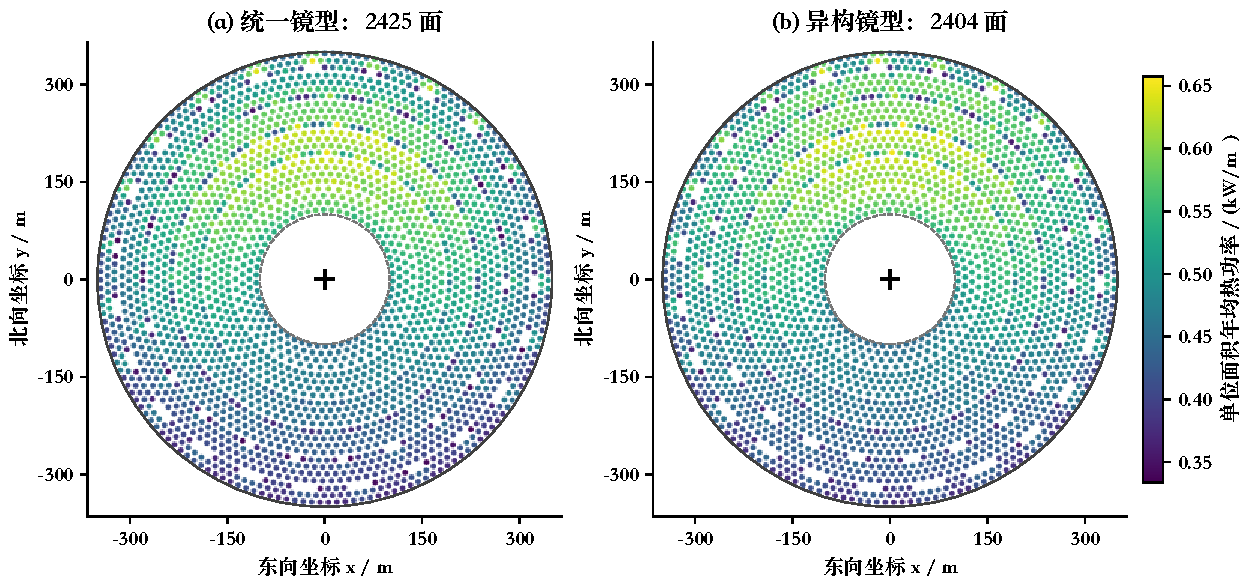
\includegraphics[width=.97\linewidth]{figures/designs.pdf}
\caption{统一镜型与异构镜型的最终布局，颜色表示逐镜单位面积年均热功率}
\label{fig:designs}
\end{figure}

相较问题一，新场采用更大的总镜面面积以满足容量。密度增加会加重遮挡，而扩大平面镜面会使接收器截断更明显，因此其单位面积功率不能简单按问题一的效率外推。优化的作用是从这些相互制约的因素中寻找容量满足后的较优面积利用方案。

图\ref{fig:designs}显示，交错环带能在维护间距约束下提供足够候选位置，收益排序删镜则对低产热区域进行选择性稀疏化。最终塔址由受限搜索确定，不能据此断言中心塔址对所有自由镜位布局都最优。

\section{问题三：分区异构镜场设计}
\subsection{变量放开与面积分配的改进方向}
异构设计保留塔址、镜数和位置变量，并把统一的 $(w,h,z)$ 扩展为逐镜 $(w_i,h_i,z_i)$。目标仍为 $\mean P/\sum_iw_ih_i$，额定功率下限不变。式\eqref{eq:constraints}中的外接圆改为 $\rho_i$，镜间距改为
\begin{equation}
\sqrt{(x_i-x_j)^2+(y_i-y_j)^2}\ge\max(w_i,w_j)+5.
\end{equation}
统一镜场本身属于异构问题的可行域，因此它是自然的初始解。但只有实际改变尺寸、高度或位置后在同一模型下提高目标，才形成有意义的第三问改进。

设某次改动使年均功率和面积变化为 $\Delta P,\Delta A$，则目标改进的精确判据为
\begin{equation}
\frac{\mean P+\Delta P}{A+\Delta A}>J
\quad\Longleftrightarrow\quad \Delta P-J\Delta A>0,
\label{eq:marginal}
\end{equation}
其中 $A+\Delta A>0$。式\eqref{eq:marginal}说明，缩小低边际产热镜面、扩大高边际产热镜面，可能改善面积利用；但 $\Delta P$ 必须包括对其他镜面遮挡的影响，不能仅按本镜面积等比例缩放。

\subsection{六分区坐标搜索与容量恢复}
对当前镜场，先计算镜心相对塔址的平面距离 $r_i$，以三分位数分为近、中、远三层，再按
\begin{equation}
b_i=\mathbf1\!\left\{|x_i-x_T|>0.7|y_i-y_T|\right\}
\end{equation}
区分侧向区域和南北向区域，组合得到六组。这一分区保留了距离与方位对效率的主要影响，同时显著降低初期搜索维度。

在原分组方案上进行高度剖面搜索。以径向三分位数为界，对中远区整体、远区单独扫描 $4.0$ 至 $6.0\,\mathrm m$、间隔 $0.5\,\mathrm m$ 的安装高度，并保留原高外圈边界构造同类候选。另比较指数为 $0.5,1,2$、外缘高度为 $4.5$ 至 $6.0\,\mathrm m$ 的平滑剖面。安装高度取候选值与 $h_i/2+0.1$ 的较大者，随后检查完整几何约束；所有方案使用同一组 $512$ 条光线和全部 $60$ 个时刻。

第三问补充搜索将容量目标提高至 $60200\,\mathrm{kW}$，以留出更大的数值裕量。高度搜索之后，对六组的镜宽、镜高与安装高度分别施加正、负扰动，一轮完整覆盖 $6\times3\times2=36$ 个候选。各候选相对同一基准构造，先剔除几何或容量不达标者，再选目标最好的可行改进。尺寸与高度步长依次为 $0.15$ 和 $0.05\,\mathrm m$，每个尺度最多执行两轮；只有整轮无改进时才记为该尺度停滞，达到轮数上限则明确记为预算停止。改变镜高时同步抬升必要的支架高度，以免把可行的增高动作误判为触地。

原方案生成阶段通过高收益区域扩高或从未占用候选位置补镜来恢复容量，补充搜索中的塔址联动也使用候选池补镜。候选次序由孤立单位面积产热提出，加入后重新计算全部镜间作用。完整双向轮次先过滤容量不足者；搜索末尾在功率富余时按收益排序删镜。目标改进动作的接受条件为
\begin{equation}
\mean P_{\rm trial}\ge P_*,\qquad J_{\rm trial}>J_{\rm current}.
\end{equation}
因此，近似收益排序只产生搜索方向，不替代最终可行性判断；最后的区域规格统一另按下述明确容差判断。

原搜索曾在 $48$ 次分组试探中接受五次改动，随后接受十二次逐镜缩高，但这只是原方案的生成记录。修正流程采用上述完整双向轮次，且塔址移动时同步平移镜位、剔除越过场界的镜面，必要时从重建候选池补镜，再复算容量，避免固定镜位导致塔周禁区试探全部失效。

为考察少数特殊镜型的必要性，最后将各组宽高统一到组内出现最多的规格，比较完整光学输出；若容量略低于搜索裕量目标，先比较整组镜高增加 $0.005$、$0.01$、$0.025\,\mathrm m$ 的恢复方案，仍不足时再尝试补镜。若规格数减少、容量仍达标且单位面积目标的相对损失不超过 $0.02\%$，则采用区域标准方案，并记录这一性能与规格数量的取舍。该容差是本文用于减少零散规格的设计选择，不是题目新增约束；平滑高度和区域镜型均需计算比较，不能预先规定其优于自由方案。

\Needspace{12\baselineskip}
\subsection{异构设计结果与两问比较}
\begin{table}[H]
\centering\small
\caption{异构镜型设计参数与范围}\label{tab:q3design}
\begin{tabular}{lrl}
\toprule
参数 & 结果 & 单位\\\midrule
吸收塔位置 & $(0.0000,\,0.2492)$ & m\\
镜面宽度范围 & 6.9402 至 7.0902 & m\\
镜面高度范围 & 6.9152 至 7.0902 & m\\
安装高度范围 & 3.5951 至 6.0000 & m\\
定日镜数目 & 2404 & 面\\
总镜面面积 & 118520.4972 & m$^2$\\
年平均输出热功率 & 60.1195 & MW\\
单位面积年平均热功率 & 0.50725 & kW/m$^2$\\
\bottomrule
\end{tabular}
\par\vspace{3pt}\begin{minipage}{.95\linewidth}\footnotesize 坐标均相对题目场地圆心；逐镜完整精度参数见随文数据。\end{minipage}
\end{table}

\begin{table}[H]
\centering\small
\caption{问题三每月 21 日平均光学效率及输出热功率}\label{tab:q3month}
\begin{tabular}{lrrrrrr}
\toprule
日期 & $\mean\eta$ & $\mean\eta_{\rm cos}$ & $\mean\eta_{\rm sb}$ & $\mean\eta_{\rm trunc}$ & $\mean P$/MW & $J$/($\unitp$)\\\midrule
1 月 21 日 & 0.47209 & 0.72040 & 0.82707 & 0.92849 & 49.3344 & 0.41240\\
2 月 21 日 & 0.50639 & 0.74013 & 0.86250 & 0.91781 & 57.1464 & 0.47771\\
3 月 21 日 & 0.52638 & 0.75999 & 0.87461 & 0.90848 & 62.6322 & 0.52357\\
4 月 21 日 & 0.54055 & 0.77734 & 0.87824 & 0.90329 & 66.5476 & 0.55630\\
5 月 21 日 & 0.54954 & 0.78674 & 0.88147 & 0.90125 & 68.6915 & 0.57422\\
6 月 21 日 & 0.55256 & 0.78958 & 0.88278 & 0.90073 & 69.3632 & 0.57983\\
7 月 21 日 & 0.54944 & 0.78664 & 0.88143 & 0.90127 & 68.6682 & 0.57402\\
8 月 21 日 & 0.53997 & 0.77667 & 0.87808 & 0.90345 & 66.3993 & 0.55506\\
9 月 21 日 & 0.52557 & 0.75899 & 0.87433 & 0.90886 & 62.3943 & 0.52158\\
10 月 21 日 & 0.50305 & 0.73763 & 0.85979 & 0.91903 & 56.3096 & 0.47071\\
11 月 21 日 & 0.46799 & 0.71872 & 0.82185 & 0.92955 & 48.5089 & 0.40550\\
12 月 21 日 & 0.44849 & 0.71187 & 0.79615 & 0.93362 & 44.8062 & 0.37455\\
\bottomrule
\end{tabular}
\par\vspace{3pt}\begin{minipage}{.95\linewidth}\footnotesize 各项效率为五个规定时刻的面积加权均值，效率无量纲；功率先逐镜求和再对时刻平均。\end{minipage}
\end{table}


\begin{figure}[htbp]
\centering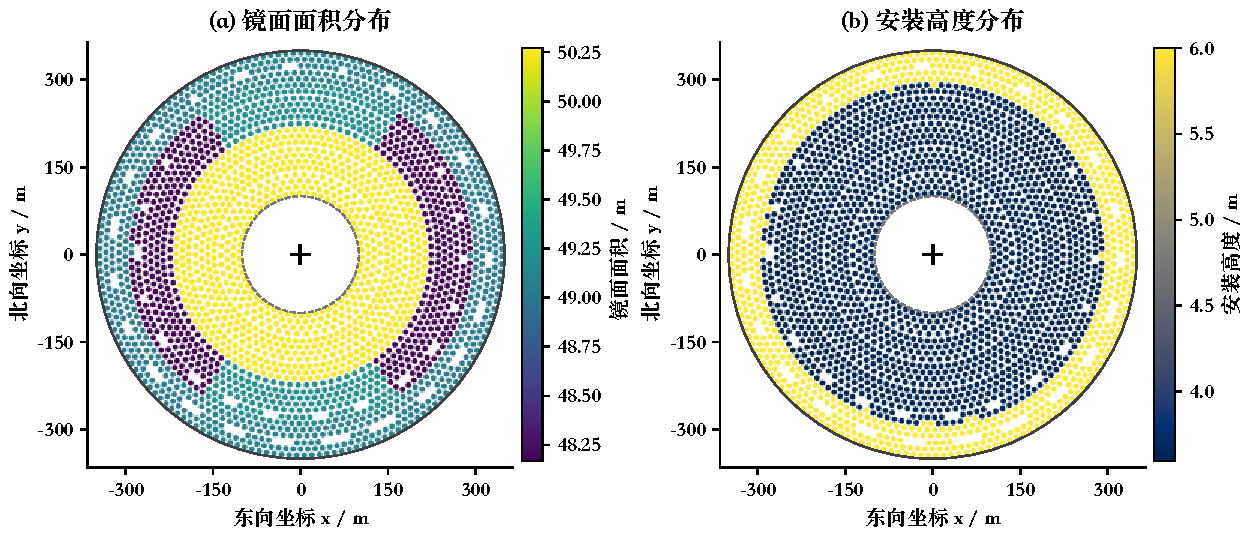
\includegraphics[width=.96\linewidth]{figures/heterogeneity.pdf}
\caption{异构设计的镜面面积与安装高度分布}
\label{fig:hetero}
\end{figure}

异构方案的参数范围见表\ref{tab:q3design}，空间分布见图\ref{fig:hetero}。最终形成 \QthreeTypes\ 种镜面宽高组合，每种至少 \QthreeMinTypeCount\ 面，安装高度共 \QthreeZTypes\ 档；高度分布由剖面比较和双向局部搜索共同确定。抬高某层可改善该层光路，也会改变它对其他镜面的遮挡，因此本模型不预设高度必须沿径向连续递增。其年均热功率为 \QthreeP\,$\mathrm{MW}$，单位面积年均输出为 \QthreeJ\,$\unitp$。相比问题二，单位面积目标提高 \GainJ\%，总镜面面积减少 \AreaSaving\%。这种收益来自尺寸、安装高度和镜面保留位置的共同变化，不能把所有提升归因于单一变量。

按相同四组全新随机种子重算原第三问方案，得到 $\RevisionOldP\,\mathrm{MW}$ 和 $\RevisionOldJ\,\unitp$。本次修正使单位面积目标再提高 $\RevisionGain\%$，配对增益的单侧 $95\%$ 下界为 $\RevisionLow\,\unitp$，表明改进并非仅由采样扰动造成。

\begin{table}[htbp]
\centering\small
\caption{三问年平均光学效率及输出热功率}\label{tab:annual}
\begin{tabular}{lrrrrrr}
\toprule
方案 & $\mean\eta$ & $\mean\eta_{\rm cos}$ & $\mean\eta_{\rm sb}$ & $\mean\eta_{\rm trunc}$ & $\mean P$/MW & $J$/($\unitp$)\\\midrule
问题一 & 0.57640 & 0.75647 & 0.91666 & 0.94844 & 35.2392 & 0.56096\\
问题二 & 0.50548 & 0.75470 & 0.84559 & 0.91328 & 60.0628 & 0.49269\\
问题三 & 0.52047 & 0.75507 & 0.86804 & 0.91270 & 60.1195 & 0.50725\\
\bottomrule
\end{tabular}
\end{table}


表\ref{tab:annual}汇总三问年均指标，对应题目要求的年平均结果表。第一问与后两问满足的容量条件不同，故主要优化比较在问题二和问题三之间进行。两问使用相同的四组独立随机种子，配对目标差的数值均值为 \PairedDiff\,$\unitp$，其单侧 $95\%$ 下界为 \PairedLow\,$\unitp$，用以检验观察到的改进是否可能仅来自采样扰动。

\begin{figure}[htbp]
\centering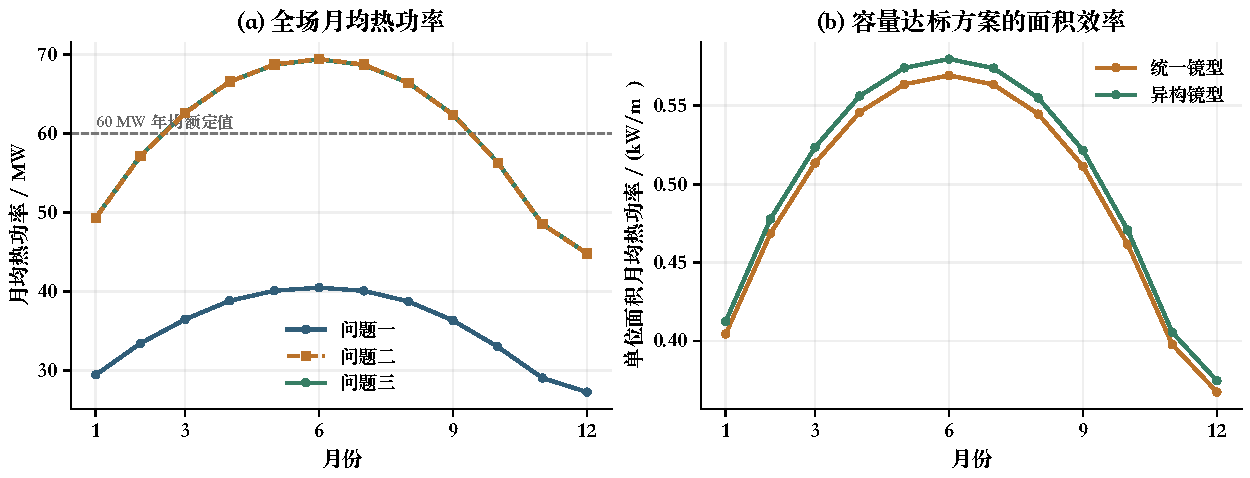
\includegraphics[width=.96\linewidth]{figures/monthly_power.pdf}
\caption{三问逐月热功率及统一、异构方案的单位面积产热比较}
\label{fig:monthly}
\end{figure}

\section{模型检验与数值误差分析}
\subsection{几何约束与能量一致性}
本次运行 $19$ 项自动检验，全部通过。检验涵盖太阳东西方向与时刻对称性、镜心反射定律、镜边水平、有限矩形边界、圆柱首次命中、逆向阴影查询、面积加权恒等式、镜序置换不变性，以及删去遮挡物后剩余镜功率不减；新增回归检验覆盖塔址与镜位联动、增高时离地约束，以及高目标但容量不足的候选不得压过可行改进。

Python/NumPy 参考实现与 C++ 加速实现分别实现光线求交，在非均匀镜面和含斜率误差的小场景中对照，光学量的绝对容差为 $2\times10^{-12}$。空间筛选结果也与全镜对追踪比较，覆盖较远反射距离情形。这里验证的是实现对所建模型的一致性，不把程序一致性等同于实测物理精度。

最终设计的主要几何裕量见表\ref{tab:constraints}。镜间距检查覆盖所有潜在冲突镜对，离地裕量是全俯仰旋转的最小间隙，场界与禁区裕量按外接圆计算，均以未四舍五入的完整参数验证。
\begin{table}[htbp]
\centering\small
\caption{最终新设计的几何约束裕量（m）}\label{tab:constraints}
\begin{tabular}{lrr}
\toprule
检查项目 & 问题二 & 问题三\\\midrule
最小镜间距余量 & 0.050024 & 0.050024\\
最小旋转离地间隙 & 0.100000 & 0.100000\\
最小场界余量 & 0.096602 & 0.105600\\
最小禁区余量 & 0.192584 & 0.192584\\
\bottomrule
\end{tabular}
\end{table}


\subsection{独立随机化下的额定功率复核}
搜索采用固定扰乱以便比较设计，但不能把经过大量试探挑出的高估结果直接作为最终结果。因此，最终另取四个独立随机种子，每组使用 $4096$ 条光线。记各组年均功率为 $P^{(1)},\ldots,P^{(M)}$，$M=4$，则
\begin{equation}
\widehat P=\frac1M\sum_{m=1}^{M}P^{(m)},\qquad
\mathrm{SE}(\widehat P)=\frac{s_P}{\sqrt M},
\end{equation}
用 Student-$t$ 分位数构造近似单侧下界
\begin{equation}
P_{\rm low}=\widehat P-t_{0.95,M-1}\frac{s_P}{\sqrt M}.
\label{eq:confidence}
\end{equation}
当 $P_{\rm low}\ge60000\,\mathrm{kW}$ 时判定通过数值容量复核。若未通过，才重新补镜恢复容量并再次精算。本次复核结果见表\ref{tab:uncertainty}。
\begin{table}[htbp]
\centering\small
\caption{四组独立随机化的年均功率复核}\label{tab:uncertainty}
\begin{tabular}{lrrrr}
\toprule
方案 & 均值/MW & 标准误/kW & 单侧 95\% 下界/MW & 额定值检查\\\midrule
问题一 & 35.23492 & 3.1505 & 35.22751 & 定场计算\\
问题二 & 60.05820 & 9.8910 & 60.03492 & 通过\\
问题三 & 60.06681 & 10.0437 & 60.04317 & 通过\\
\bottomrule
\end{tabular}
\par\vspace{3pt}\begin{minipage}{.95\linewidth}\footnotesize 每组每镜每时刻 4096 条光线；区间仅表示随机化数值积分的不确定性。\end{minipage}
\end{table}


式\eqref{eq:confidence}使用独立扰乱组之间的离散程度，而不是将同一 Sobol 序列中的每条光线视为独立样本。由于独立组数有限，且随机化积分的分布未被严格证明为正态，这一 $t$ 下界是近似数值不确定性指标；它不包含太阳模型、天气、制造与安装误差。

\subsection{光线数收敛与旧近似模型对照}
固定最终布局与一组独立种子，分别使用 $128$、$512$、$1024$、$2048$ 和 $4096$ 条光线，保持 Sobol 点的嵌套结构。表\ref{tab:convergence}给出年均热功率，最后一列为四组 $4096$ 条光线的最终均值。
\begin{table}[htbp]
\centering\small
\caption{不同光线数下的年均热功率（MW）}\label{tab:convergence}
\begin{tabular}{lrrrrrr}
\toprule
方案 & 128 & 512 & 1024 & 2048 & 4096 & 最终均值\\\midrule
问题一 & 35.0005 & 35.2428 & 35.2593 & 35.2643 & 35.2428 & 35.2392\\
问题二 & 60.3994 & 59.9718 & 60.0527 & 60.0404 & 60.0620 & 60.0628\\
问题三 & 60.3802 & 60.0264 & 60.1116 & 60.1055 & 60.1176 & 60.1195\\
\bottomrule
\end{tabular}
\end{table}


\begin{figure}[H]
\centering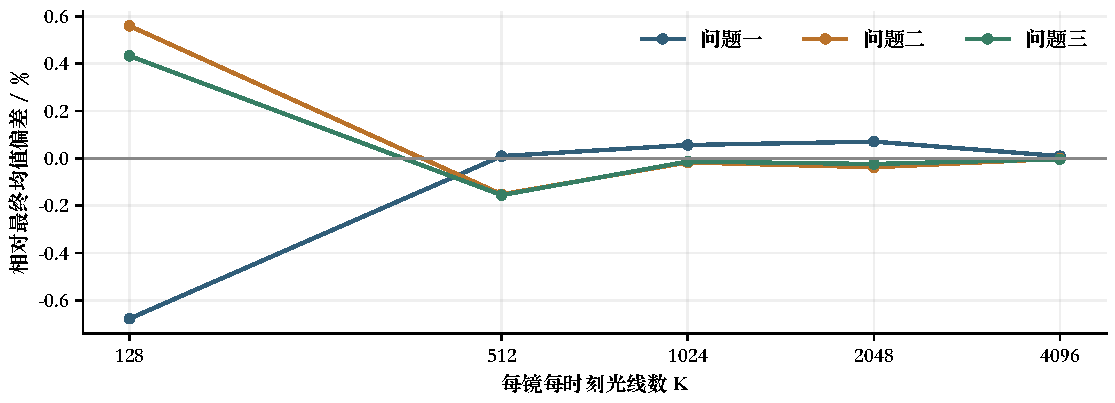
\includegraphics[width=.93\linewidth]{figures/convergence.pdf}
\caption{不同光线数下相对最终四组均值的数值偏差}
\end{figure}

收敛误差不必逐级单调减小，因为求交指示函数在几何边界处不连续；重点是较高光线数的结果是否稳定，以及独立随机化估计是否明显小于设计的额定功率裕量。三问中 $4096$ 条光线单组相对四组均值的最大偏差为 \ConvMax\%。

另外，将固定损失率方法生成的对照方案放入当前光学模型进行同口径评价。该方案有 $1589$ 面 $8\,\mathrm m\times8\,\mathrm m$ 镜，按阴影遮挡效率恒为 $0.95$、截断效率恒为 $0.90$ 选镜时，估计年均功率约 $60.006\,\mathrm{MW}$；当前模型复算得到 \LegacyP\,$\mathrm{MW}$。这一差别表明，容量约束附近的设计必须使用与论文一致的光学模型重新验证，固定损失率的容量估计不能直接迁移到几何追踪模型。

\section{物理假设敏感性分析}
\subsection{情景设置与评价指标}
保持最终镜场设计固定，分别改变塔身半径、太阳视半径和镜面斜率误差。塔身半径取 $0$ 和 $3\,\mathrm m$，其中 $0$ 表示去掉塔身而仍保留集热器本体；太阳视半径取 $4.2$ 和 $5.1\,\mathrm{mrad}$；斜率误差取 $0.5$ 和 $1.0\,\mathrm{mrad}$。

斜率误差情景在镜面局部两个切向方向加入独立零均值高斯扰动，标准差为给定 $\sigma$，截断到 $\pm4\sigma$ 后重新归一化法向。该情景表达局部面形或指向扰动对光斑扩展的影响，不把其视为题目给定制造精度。

各情景用相同的 $1024$ 条光线和相同随机种子，按
\begin{equation}
\Delta_{\rm rel}=100\%\times\frac{P_{\rm scenario}-P_{\rm baseline}}{P_{\rm baseline}}
\end{equation}
计算配对功率变化。基准也在同样的 $1024$ 条光线下重算，避免把采样精度变化混入物理参数影响。

\begin{table}[htbp]
\centering\small
\caption{物理假设变化引起的年均热功率相对变化}\label{tab:sensitivity}
\begin{tabular}{lrrr}
\toprule
相对基准的扰动 & 问题一 & 问题二 & 问题三\\\midrule
无塔身（半径 0 m） & +0.028\% & +0.028\% & +0.028\%\\
塔身半径 3 m & -0.016\% & -0.015\% & -0.015\%\\
太阳视半径 4.2 mrad & +0.579\% & +0.745\% & +0.753\%\\
太阳视半径 5.1 mrad & -0.642\% & -0.814\% & -0.821\%\\
斜率误差 0.5 mrad & -0.512\% & -0.511\% & -0.517\%\\
斜率误差 1.0 mrad & -1.994\% & -2.238\% & -2.255\%\\
\bottomrule
\end{tabular}
\par\vspace{3pt}\begin{minipage}{.95\linewidth}\footnotesize 固定最终布局；所有情景与各自基准均采用同种子的 1024 条光线。\end{minipage}
\end{table}


\subsection{结果解释与设计含义}
塔身半径增大主要改变低太阳高度时的阴影与接收器下方的遮挡，影响集中在与塔身投影相交的镜面；其对全场均值的影响随布局而变。太阳视半径扩大使入射角分布更宽，反射光束在接收器处进一步扩展，通常增加边缘溢出；但个别光线也可能从原先未命中转为命中，因此必须整体积分。

镜面斜率误差经反射角近似放大两倍，远距离镜面的光斑位移更显著。当人为增大斜率误差后功率下降超过搜索预留的数值裕量时，原方案可能不再满足 $60\,\mathrm{MW}$。这并非数值复核失效，而是物理假设发生了变化。因而本文的最终达标结论严格针对所列基准假设；若用于实际电站，应引入实测太阳形状、塔身几何与制造误差，并据此增加容量储备或重新优化。

\section{模型评价与结论}
\subsection{模型的特点}
本文的主要特点是把入射可见性、反射可见性和接收器命中统一到逐光线能量中。效率分解能够精确还原所计算功率，重叠阴影按并集处理，条件截断与遮挡保持相关。有限矩形和有限圆柱求交则保证了镜边与集热器尺寸真正参与计算。

求解方面，容量筛选减少明显无望候选的成本，收益排序删镜具有固定采样下的可行性依据，分区搜索使第三问高维自由度能够被逐步利用。精算结果和几何约束分开复核，配对随机化又使两问间的小幅目标差具有可检验的数值依据。

\subsection{适用范围与改进方向}
第一，太阳盘、塔身半径和有效受光面属于显式物理假设，尚未通过实际电站数据校准。第二，优化只搜索三类参数化布局及其局部改动，且本次从已有检查点继续搜索、每尺度轮数有限；不能据此宣称对所有塔址、镜位和逐镜尺寸得到全局最优。第三，四组随机化提供的是有限样本的数值误差估计，对更小的优化收益应增加独立组数。

后续可在保持同一光学评价器的基础上，增加更自由的位置交换与连续镜位优化，或按边际产热而非仅按径向分组调整镜型；也可引入天气概率、反射率衰减和制造成本，将单位面积产热扩展为实际年发电量或经济性目标。这些改进需要新增数据和搜索预算，不影响本文对题目规定基准的结果报告。

\subsection{结论}
在题目规定的时刻、场地和设备参数下，联合光线能量积分模型给出附件镜场年均热功率 \QoneP\,$\mathrm{MW}$。统一镜型设计与异构设计分别达到 \QtwoP\,$\mathrm{MW}$ 和 \QthreeP\,$\mathrm{MW}$，独立数值复核的单侧下界均超过 $60\,\mathrm{MW}$，几何约束全部满足。异构设计将单位面积年均热功率提高至 \QthreeJ\,$\unitp$，较统一镜型提升 \GainJ\%。结果支持在额定容量约束下，通过实际光路评价与分区面积调整改善镜场设计。

\begin{thebibliography}{9}
\small
\bibitem{problem} 全国大学生数学建模竞赛组委会. 2023年高教社杯全国大学生数学建模竞赛A题：定日镜场的优化设计及附件[Z]. 2023.
\bibitem{zhang} 张平等. 太阳能塔式光热镜场光学效率计算方法[J]. 技术与市场, 2021, 28(6): 5--8.
\bibitem{farges} Farges O, Bézian J J, El Hafi M. Global optimization of solar power tower systems using a Monte Carlo algorithm: Application to a redesign of the PS10 solar thermal power plant[J]. Renewable Energy, 2018, 119: 345--353.
\bibitem{sobol} Sobol' I M. On the distribution of points in a cube and the approximate evaluation of integrals[J]. USSR Computational Mathematics and Mathematical Physics, 1967, 7(4): 86--112.
\bibitem{owen} Owen A B. Scrambled net variance for integrals of smooth functions[J]. The Annals of Statistics, 1997, 25(4): 1541--1562.
\end{thebibliography}

\clearpage
\appendix
\section{实验数据与复现说明}
\subsection{文件与精度约定}
论文数据由当前仓库的 \texttt{heliostat} 模块直接计算，未修改核心物理公式和光线追踪程序。\texttt{final/reoptimize.py} 保存补充搜索的基准快照与记录；\texttt{final/reproduce.py} 固定恢复参数、容量裕量和独立复核种子，并将输出写入 \texttt{final/data/}。文中的表格由 \texttt{build\_assets.py} 从该目录读取，图形亦直接使用逐镜或逐时刻数组生成。

\begin{table}[H]
\centering\small
\caption{随文实验文件索引}
\begin{tabular}{p{62mm}p{86mm}}
\toprule
文件 & 内容\\\midrule
\texttt{q1.npz, q2.npz, q3.npz} & 三问镜场的完整精度坐标、宽高与塔址\\
\texttt{q1\_optics.npz} 等 & 逐镜、逐时刻效率与热功率\\
\texttt{metrics.csv} & 三问逐月平均结果，包含题目要求的效率与功率\\
\texttt{instantaneous.csv} & 全部 $60$ 个时刻的场均指标\\
\texttt{result2.csv, result3.csv} & 按题目八列字段顺序保存的逐镜设计参数\\
\texttt{verification.json} & 年均结果、独立随机化误差、约束裕量、输入与源码哈希\\
\texttt{convergence.json} & 五级光线数下的收敛结果\\
\texttt{sensitivity.json} & 六种物理假设扰动的同种子配对结果\\
\texttt{q2\_restart\_history.json} 等 & 塔址重启、高度剖面及完整双向轮次的实际记录\\\bottomrule
\end{tabular}
\end{table}

正文尺寸一般保留四位小数，效率和功率的显示精度按表头约定，计算与约束检验始终使用未舍入数组。逐镜文件的八列依次为吸收塔 $x$ 坐标、吸收塔 $y$ 坐标、定日镜序号、镜面宽度、镜面高度、镜心 $x$、镜心 $y$、镜心 $z$ 坐标。用于正式提交时，可将数值按同一字段顺序写入题目要求的 \texttt{result2.xlsx} 和 \texttt{result3.xlsx}，不要用正文舍入值反推镜心位置。

\subsection{计算步骤}
在项目根目录、已安装仓库依赖的 Python 环境中运行：
\begin{verbatim}
python -m unittest discover -s tests -v
python final/reproduce.py
python final/build_assets.py
cd final
latexmk -xelatex paper.tex
\end{verbatim}
已有最终数组时上述命令重做独立验证。补跑本文修正搜索可先执行 \texttt{python final/reoptimize.py q2} 和相应的 \texttt{q3} 命令，它们读取保留的审计前快照；再按上述流程复核与编译。空数据目录则从恢复参数执行新版完整搜索，路径不同，不保证重现同一局部解。搜索使用种子 $202309$；修正版最终复核改用 $1915721$、$1916718$、$1917715$、$1918712$，避免重复使用诊断阶段参与比较的种子。所有输入文件的 SHA-256 在运行前后比较，确保题目附件未被改写。

\section{核心求解伪代码}
\begin{table}[H]
\centering\small
\begin{tabular}{p{150mm}}
\toprule
\textbf{算法 A：镜场光学评价}\\\midrule
输入镜心、尺寸、安装高度、塔址、太阳与接收器参数；生成联合 Sobol 样本。\\
对每个规定时刻：计算太阳方向、$\DNI$、镜面法向和水平局部坐标系。\\
依据镜面高度界与光锥包络建立潜在遮挡邻居列表。\\
对每面镜、每个联合采样点：计算镜面点、入射方向和反射方向。\\
朝向太阳查询阴影；沿反射方向查询镜面、塔身与有限集热器首次相交。\\
按光线权重累加 $C,S,H$，得到条件效率和单镜功率。\\
先逐镜汇总功率，再按五时刻和六十时刻平均；效率按面积加权。\\
输出逐镜、逐时刻与月均、年均指标。\\\bottomrule
\end{tabular}
\end{table}

\begin{table}[H]
\centering\small
\begin{tabular}{p{150mm}}
\toprule
\textbf{算法 B：统一镜型与异构镜型优化}\\\midrule
恢复已有可行布局参数并重新计算完整光学容量，设置目标 $P_*=60150\,\mathrm{kW}$。\\
对统一镜型补充塔址与相位多起点搜索，每次重建镜位，精算后与基准比较。\\
对每个试探生成镜场，检查约束；完整追踪后按面积收益排序删镜并重算。\\
仅接受功率达到 $P_*$ 且单位面积目标增加的方案，得到问题二设计。\\
第三问取 $P_*=60200\,\mathrm{kW}$，从既有异构方案比较分组高度剖面。\\
按完整正负轮次调整组内宽高与安装高度；容量富余时删镜。\\
联动移动塔址与镜位，必要时补镜；比较区域标准镜型并记录性能取舍。\\
用独立随机化精算两问；检查约束、功率下界及配对单位面积目标差。\\
输出最终设计、收敛结果与假设敏感性结果。\\\bottomrule
\end{tabular}
\end{table}

\end{document}
